\documentclass[a4paper]{book}

\usepackage[english]{babel}
\usepackage[utf8]{inputenc}
\usepackage[T1]{fontenc}
\usepackage{lmodern}

\newcommand{\Author}{Sebastian Einsiedler}
\newcommand{\Title}{Settlers or cultures like game}

\title{\Title}
\author{\Author}

\usepackage{amsmath, amssymb}
\usepackage{enumerate}
\usepackage{xcolor}
\usepackage{hyperref}
\hypersetup{
	bookmarks=true,
	unicode=true,
	pdfauthor = {\Author},
	pdftitle = {\Title},
	pdfsubject = {\Title},
	pdfsubject = {\Author, \Title, Game development},
	colorlinks = true,
	linkcolor = {blue!50!black},
	filecolor = {red!50!black},
	urlcolor = {blue!75!black}
}
\usepackage{csquotes}

\usepackage{footnotebackref}
\usepackage{longtable}
\usepackage{booktabs}
\usepackage{graphicx}
\usepackage[singlespacing]{setspace}
\usepackage[toc]{glossaries}
\usepackage{pdflscape}
\usepackage{tikz}
\usetikzlibrary{positioning}
\tikzset{
	% The raw resources that renew like game or trees
	raw_renewable/.style={
		draw=green,rectangle
	},
	% The raw resources that are limited like ore or stone
	raw_limited/.style={
		draw=gray,rectangle
	},
	% The livestock
	livestock/.style={
		draw=red,rectangle
	},
	% The resources that are only obtained by farming
	produce/.style={
		draw=yellow,rectangle
	},
	% The intermediate products
	intermediate/.style={
		draw=blue,rectangle
	},
	% The building material
	material/.style={
		draw=black,rectangle
	},
	% The finished foods
	food/.style={
		draw=green!50!yellow,rectangle
	},
	% Normal goods
	good/.style={
		draw=purple,rectangle
	},
	% Normal goods
	tool/.style={
		draw=purple!50,rectangle
	},
	% The luxury goods
	luxury/.style={
		draw=yellow!50,rectangle
	},
	% Weapons
	weapon/.style={
		draw=red!50,rectangle
	},
}

\makeglossaries{}

\newglossaryentry{Vikings}{
	name=children of the spirits,
	description={simple nature loving craftsmen,
		with a strong connection to the land and nature that surrounds them}
}
\newglossaryentry{Nomads}{
	name=mounted men,
	description={fierce warriors and raiders, that raise large herds and conquer their foes
		on the back of their mounts with their cruel gods and the wind in their back}
}
\newglossaryentry{Egyptians}{
	name=river folk,
	description={erect great monuments within fertile river plains.
	They fight for the glory of their kings and an immortal afterlife.}
}
\newglossaryentry{Aztecs}{
	name=servants of the serpent,
	description={need to feed the sky serpent with human sacrifice so it can then be
		consumed by sun.
		Born from corn and water they are constantly on the search for new sacrifices.
		For the serpent hungers and if you do not feed it, it will consume you}
}
\newglossaryentry{Japanese}{
	name=empire,
	description={lies within the fertile plains-
		Its peasants grow rice, its craftsman forge tools and weapons,
		so its priest and artists can create great works for the celestial dragons.
		Its warriors defend the borders with bow, katana and musket against all invaders}
}
\newglossaryentry{Romans}{
	name=republics,
	description={stand against the gods.
	Where other chose slavery in the face of the supernatural the republics chose industry and science.
	Heavily armored its legions advance towards its enemy,
	while the mortars turn fertile plains into burning hell.
	The complex bureaucracy and trade deals enable the republics to field
	powerful legions commanded by officers and supported by fearsome war-machines,
	to lay low all that oppose the might of humanity}
}

\begin{document}

\maketitle

\tableofcontents

\chapter{The tribes}
This chapter describes the different human factions inhabiting the world.
It describes their economy, religion culture and play-style.
Each faction is centred around a unique play-style with partly overlapping good production,
with the other factions.

\section{\Gls{Vikings}}

	\begin{flushright}
		\emph{One with the spirits, one with nature.}
	\end{flushright}

	Deep within the woods, the blooming meadows live the \gls{Vikings}.
	They have a close connection to nature and its spirits,
	which they venerate in special sanctuaries.

	In the forest their hunters stalk deer and boars,
	among the druids and foragers.
	The foragers collect herbs and mushrooms for the production
	of medicine and (herb) flavored mead and mushroom ale.
	The wheat for the ale is grown in small fields in front of their towns,
	where their craftsmen produce golden-jewelry, drinking horns, pillows,
	woolen clothes, candles, leather shoes and wooden and metal tools.
	To feed them the backers bake bread and delicious chestnut- and apple pies.
	Should the miller be sick, the instead feast on meat, fish and apples.

	Their houses are built from timber, boards and stones.
	Their hamlets protected by simple palisades,
	their villages by wooden walls and towers and their cities by stone walls, towers
	and the spirits the so cherish.

	While the fish are caught on the shore, sheep and oxen
	are raised on the meadows and chicken and pigs fed with wheat and chestnuts.
	Behind the pastures, wheat-fields and orchards you can find the mountains.
	If they do not turn them into sacred hallowed places,
	they mine for copper, iron, gold and coal.
	They use this metals to make various tool.
	The most beloved of this tools is the ax, used by their lumberjacks,
	the butchers and the warriors alike.

	If the wood-burner works diligently and enough metal is found in the mountain,
	their weapon smith will forge battle-axes, spears and swords.
	Luckily he also works as a bow-maker on the side supplying them with short bows.

	Tho protect their warriors they manufacture medium wooden and medium metal shields,
	leather and light metal armor.
	To protect the heads of their warriors they use leather caps, helmets and horned helmets.
	The latter one are seen as quite prestigious among them and are given to the most important
	warriors to boost their morale in battle.

	\subsection{Religion}
		The \gls{Vikings} dedicate areas to the spirits.
		Within theses areas the spirits prosper and supply the \gls{Vikings}
		with resources and protect these sacred places,
		while they remain pristine.
		The sanctuaries have a inner circle and an outer circle.
		One sanctuaries outer circle can not overlap with the outer circle of another sanctuary.

		All sanctuaries are employ druids.
		They improve the sanctuary and collect magical resources from it.
		In the druid-circle great druids can be trained.
		These can then use the collected magical resources to weave spells.

		\subsubsection{Sanctuary of the forest}
			The spirits of the forest cherish the trees and the sanctuary is strengthen by
			all ancient trees in its inner and outer circle.
			The druids plant trees in the inner and outer circle of the sanctuary,
			which produce magical resource.

			\paragraph{Level 0: Sacred grove}
				After the sanctuary was established the trees around it slowly turn into ancient trees.
				Druids can harvest ancient bark from this trees\footnote{
					Magic bark is just magic resource, not a special good.
				}.
				Great Druid can use the spell \textquote{Create forest}\footnote{
					A small forest appears at the target area of the spell.
				} once the sanctuary was established.

			\paragraph{Level 1: Living woods}
				Additional herbs and mushrooms begin to sprout in the inner and outer circle
				of the sanctuary.
				A bear appears to defend the inner circle of the sanctuary.
				Boars and deer appear in its inner circle regularly.
				Great druids can use the spell \textquote{Animal kinship}\footnote{
					Creates a number of boars and deer at the place.
				} once this level is reached.

			\paragraph{Level 2: Ancient forest}
				Ancient trees now grow chestnuts and apples.
				Wisps start appearing confusing and stunning enemies walking into the inner circle
				of the sanctuary.
				The wisps also leave gits of mushrooms and herbs at the center of the sanctuary.
				Great druids can use the spell \textquote{Wisp lights}\footnote{
					A few lights appear stunning enemy soldiers.
				} once this level is reached.

			\paragraph{Level 3: Enchanted woods}
				The sanctuary attracts a might ent.
				The tree-shepherd patrols the inner circle of the sanctuary
				and kills enemies that dare to venture in it.
				He also delivers the dead-wood of the forest as timber to its center.
				Thorns fill out the entire inner circle of the forest,
				injuring all enemies that walk upon it.
				Great druids can use the spell \textquote{The forests revenge}\footnote{
					Trees within the area of the spell awakened.
					They maul close enemies and throw branches at them over a short distance.
				} once this level is reached.

		\subsubsection{Sanctuary of the meadows}
			The spirits of the meadows cherish all flowers on it.
			The druids fell trees, remove rocks and plant flowers
			within the inner and outer ring of the sanctuary.

			\paragraph{Level 0: Peaceful fields}
				Once the sanctuary was established the flowers begin to bloom.
				From these blooming flowers the druids can harvest the enchanted petals{
					Enchanted petals are just magic resource, not a special good.
				}.
				Great Druid can use the spell \textquote{Spring}\footnote{
					A bunch of flowers appear.
					Since this is the only way besides the sanctuary to create flowers
					it is a convenient way to either level it up faster or
					get mead production going.
				} once the sanctuary was established.

			\paragraph{Level 1: Flower fields}
				A wild bull appears defending the inner circle of the sanctuary.
				The grass grows lusher and sheep and oxen grow faster on the meadow.
				Great druids can use the spell \textquote{The great shedding}\footnote{
					All sheep in the area of the spell immediately produce two units of wool.
				} once this level is reached.

			\paragraph{Level 2: Fairy circle}
				A bunch of fairies fly between the flowers, in the inner circle.
				They can turn enemies into sheep for a short duration.
				They also assist the bees collecting honey,
				while shearing the sheep delivering honey and wool to the center of the sanctuary.
				Great druids can use the spell \textquote{Bee hive}\footnote{
					A swarm of bee appears and chases enemies in a random direction,
					while doing minor damage to them.
				} once this level is reached.

			\paragraph{Level 3: Unicorn pasture}
				A herd of unicorns moves into the inner circle of the sanctuary.
				The will trample and pierce unwelcome intruders with their horns.
				They shed their horns on occasion leaving them in the center of the
				sanctuary.
				Once the herd grows above a certain size unicorns will join the \gls{Vikings}
				as mount to defend the spirits.
				Great druids can use the spell \textquote{Unicorn stampede}\footnote{
					Calls a herd of unicorns from the spirit realm,
					that trample from the position of the great druid
					in the direction of the spell.
					Trampling all in their way.
				} once this level is reached.

		\subsubsection{Sanctuary of the sea}
			This has to be built within a lake or the sea shore.
			The spirits of the sea cherish the rough waves and the cold breeze.
			The druids transform adjacent land into swamp and row out
			to the sea in boat to converse with dolphins and manatees.

			\paragraph{Level 0: Salty rocks}
				Once the sanctuary was established the water tiles around it slowly
				become rough waves.
				Willows grow in the swamp.
				From willows the and rough seas the druids can bottle wailing{
					Bottled wailing is just magic resource, not a special good.
				}.
				Great Druid can use the spell \textquote{Rich fishing grounds}\footnote{
					The number of fish in the water increases,
				} once the sanctuary was established.

			\paragraph{Level 1: Great reef}
				Countless fish now live in the reef\footnote{
					Fish spawn next to the sanctuary.
				}
				and only kept in the balance by a large shark that circles it within the inner circle.
				In the swamp within the inner circle a giant toad preys on the enemies of the \gls{Vikings}.
				Great Druid can use the spell \textquote{Salty catch}\footnote{
					Used on the coast, it creates a bunch of salt and fish.
				} once this level is reached.

			\paragraph{Level 2: Undersea harbor}
				The spirits of the sea walk on the land.
				Within the inner sanctuary a guard of fish-men defends the sanctuary
				with their spears fashioned from (whale)-bone.
				They gift the druids gold in exchange for their stories.
				Great Druid can use the spell \textquote{Wet warriors}\footnote{
					Used on the coast it calls a few fish-men,
					that attack nearby enemies before retreating back into the depths.
				} once this level is reached.

			\paragraph{Level 3: Temple of the nymph}
				A nymph has moved into the sanctuary.
				Her beauty enchanting all that see her.
				If enemies are foolish enough to attack her,
				she will graciously accept a few of them as her new honor-guard.
				They will defend her against their former comrades until they die of
				starvation.
				She will also gift a Mithril sword to the \gls{Vikings} from time to time
				to thank them for the protection of the sanctuary.
				Great Druid can use the spell \textquote{Sirens song}\footnote{
					Used on the coast it calls all enemies towards the shore,
					where they strip themselves of weapons and armor
					and start to swim towards the siren until they drown.
				} once this level is reached.

		\subsubsection{Mountain sanctuary}
			This has to be built next to mountain and rocks.
			The spirits appreciate rock carvings and moss.
			The druids carve runes on rocks or lift rocks from the ground\footnote{
				Since rocks yields stone this should be a very slow process.
			}.

			\paragraph{Level 0: Rock field}
				Once the sanctuary was established crystals start to sprout on the carved rocks.
				The light of this crystals can be harvested by the druids{
					This yields magic resource.
				}.
				Great Druid can use the spell \textquote{The bones of the earth}\footnote{
					A bunch of rocks appear in the target area.footnote{
						These can be harvested for stone.
					}
				} once the sanctuary was established.

			\paragraph{Level 1: Crystal grotto}
				A lonely cougar moves into the inner circle of the sanctuary.
				It attacks all enemies of the \gls{Vikings}.
				Carved-Rocks covered in crystals, explode after a time,
				yielding a small amount of stone.
				Great Druid can use the spell \textquote{Riches of the mountain king}\footnote{
					The resources of mines in the area are increased by a small amount.
				} once this level is reached.

			\paragraph{Level 2: Troll cave}
				A mighty troll moves in.
				With his mighty pick the troll not only keeps the inner circle save of invaders,
				but also mines the occasional piece of copper ore from the crystals depositing it its hoard
				in the center of the sanctuary.
				Great Druid can use the spell \textquote{You shall be stone}\footnote{
					Turns a small amount of enemies and their weapons permanently into stone/rocks.
					So the houses of the \gls{Vikings} can be built from their enemies.
				} once this level is reached.

			\paragraph{Level 3: Dragon peak}
				A mighty dragon takes the center of the sanctuary as its domain.
				It defends the inner sanctuary with its flaming breath from invaders
				and permits the druids to collect its iron scales once they shed.
				Great Druid can use the spell \textquote{Dragons curse}\footnote{
					Turns a small amount of enemies and their weapons permanently into copper-, gold- and iron-bars.
				} once this level is reached.

		\subsubsection{Sanctuary of the hearth fire}
			The spirits of the hearth fires love the \gls{Vikings}, their fields and houses\footnote{
				The sanctuary levels with wheat fields and buildings in its inner and outer circle.
				Making it different other sanctuaries.
			}.
			The druids walk from house to house lighting candles\footnote{
				So this is the only sanctuary that consumes resources.
			} to delight the spirits.

			\paragraph{Level 0: Hamlet}
				Once the sanctuary was established the burnt candles turn into spirit-embers,
				which can be collected by the druids\footnote{
					Spirit embers are magical resource not a special good.
				}.
				Great Druid can use the spell \textquote{Wonderful harvest}\footnote{
					A bunch of ready to harvest wheat appears.
				} once the sanctuary was established.

			\paragraph{Level 1: Village}
				A group of mocking spirits appear and wander the inner circle of the sanctuary.
				Their mocking distracts enemies stopping them from attacking.
				All shops and fields passed by the spirits gain a production boost.
				If the spirits pass an empty pigsty or chicken-pen a pig or chicken appears in it.
				Great Druid can use the spell \textquote{Spirits gifts}\footnote{
					A bunch of clothes and bread appear.
				} once this level is reached.

			\paragraph{Level 2: Town}
				A ghostly night-watch appears and defends the inner circle against intruders at night.\footnote{
					The night-watch are ghostly soldiers armed with spears.
				}.
				At dawn the night watch turns into alcoholic beverages.
				During the day a burning knight walks through the inner circle of the sanctuary.
				Ready to defend it against invaders.
				At dusk the knight turns into a few units of coal. 
				Great Druid can use the spell \textquote{Black rider}\footnote{
					A black ghostly rider appears.
					Slaying one enemy, causing nearby enemies to flee in panic.
				} once this level is reached.

			\paragraph{Level 3: City}
				A group of animated armor suites patrols the inner circle of the sanctuary\footnote{
					They wear metal armor, helmets and either bows or swords and shields.
				}.
				From time to time the armors are remade by the sanctuary leaving their
				components behind for the warriors of the \gls{Vikings}.
				Great Druid can use the spell \textquote{The great bell}\footnote{
					A giant bell tolls three times shattering walls beneath it.
				} once this level is reached.

	\subsection{Starting conditions}
		The \gls{Vikings} start with a great wooden hall.
		This is the center of their community, where they can store resources
		and train warriors.
		The balconies of the hall can also be manned by bowmen and the doors locked
		Turning this building in a defensive point.

	\subsection{Play-style}
		They are rather generic, growing food, mining for ore, felling trees.
		Their gimmick are the sanctuaries, forcing them to carefully consider the use of their territory.
		The sanctuaries give them a great natural defense and infinite resources for little work.
		On the offensive they can rely on their medium warriors,
		but are better of to use the spells of their great druids.
		In the early game they can use their tool-smithy to forge axes and start raiding their neighbors,
		before those build a working weapon production line.
		For siege-warfare they rely on ladders and \textquote{The great bell}-spell.
		With their ability to build longboats and upgrade their buildings from simple tents,
		to huts, to wooden houses  and then to stone houses, they are quite static.
		They usually defend themselves with palisades, wooden walls and towers and in the
		late game with stone walls.

		Their true weakness is the desert, because they have neither sanctuary nor use for it.
		They can also only farm on rare fertile soil and their yields are small compared to
		other people.

	\subsection{Resource-flow}
		How the resources flow through the economy of the \gls{Vikings}.
		These are organized according to the final product.

		\autoref{meat}

	\begin{figure}[h]
		\centering
		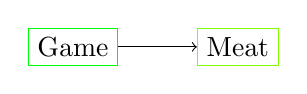
\begin{tikzpicture}
			\node [raw_renewable] (Game) at (0,0) {Game};
			\node [food] (Meat) [right=of Game] {Meat};
			\draw [->] (Game) -- (Meat);
		\end{tikzpicture}
		\caption{Meat-production}\label{meat}
	\end{figure}

	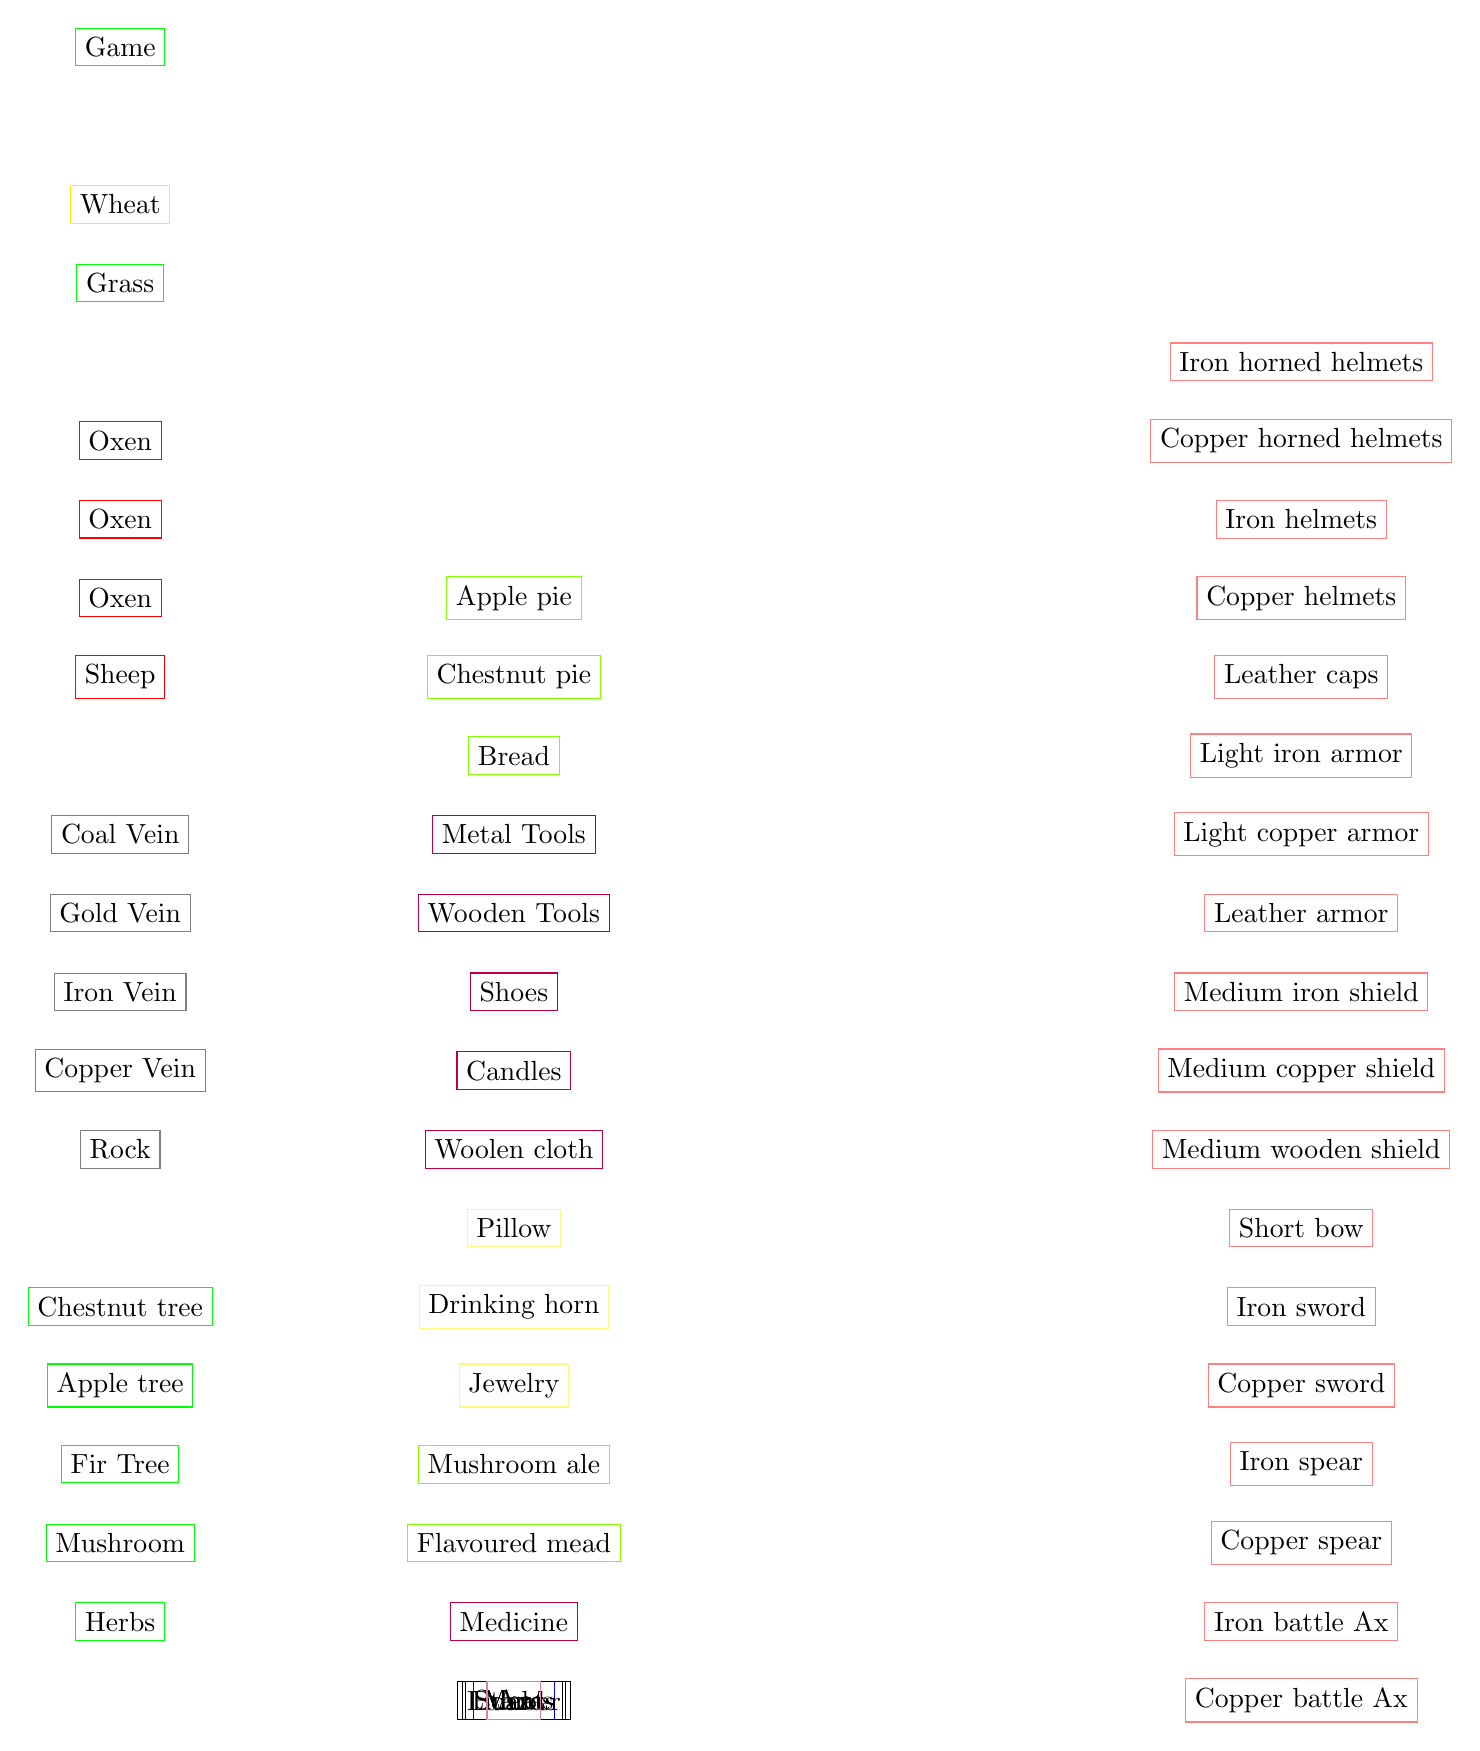
\begin{tikzpicture}
		\node [raw_renewable] (Herbs) at (0,1) {Herbs};
		\node [raw_renewable] (Mushroom) at (0,2) {Mushroom};
		\node [raw_renewable] (Fir Tree) at (0,3) {Fir Tree};
		\node [raw_renewable] (Apple trees) at (0,4) {Apple tree};
		\node [raw_renewable] (Chestnut trees) at (0,5) {Chestnut tree};
		% Ores
		\node [raw_limited] (Rock) at (0,7) {Rock};
		\node [raw_limited] (Copper Vein) at (0,8) {Copper Vein};
		\node [raw_limited] (Iron Vein) at (0,9) {Iron Vein};
		\node [raw_limited] (Gold Vein) at (0,10) {Gold Vein};
		\node [raw_limited] (Coal Vein) at (0,11) {Coal Vein};

		% Livestock
		\node [livestock] (Sheep) at (0,13) {Sheep};
		\node [livestock] (Oxen) at (0,14) {Oxen};
		\node [livestock] (Chicken) at (0,15) {Oxen};
		\node [livestock] (Pig) at (0,16) {Oxen};

		% Produce
		\node [raw_renewable] (Grass) at (0,18) {Grass};
		\node [produce] (Wheat) at (0,19) {Wheat};

		% The sea
		\node [raw_renewable] (The sea) at (0,21) {Game};


		\node [food] (Meat) at (5,0) {Meat};
		\node [food] (Fish) at (5,0) {Meat};
		\node [intermediate] (Flour) at(5,0) {Meat};
		\node [material] (Lumber) at(5,0) {Lumber};
		\node [material] (Boards) at(5,0) {Boards};
		\node [material] (Stones) at(5,0) {Stones};
		\node [tool] (Ax) at(5,0) {Ax};
		\node [good] (Medicine) at (5,1) {Medicine};
		\node [food] (Flavoured mead) at (5,2) {Flavoured mead};
		\node [food] (Mushroom ale) at (5,3) {Mushroom ale};
		\node [luxury] (Jewelry) at (5,4) {Jewelry};
		\node [luxury] (Drinking horns) at (5,5) {Drinking horn};
		\node [luxury] (Pillow) at (5,6) {Pillow};
		\node [good] (Woolen clothes) at (5,7) {Woolen cloth};
		\node [good] (Candles) at (5,8) {Candles};
		\node [good] (Shoes) at (5,9) {Shoes};
		\node [good] (Wooden Tools) at (5,10) {Wooden Tools};
		\node [good] (Metal Tools) at (5,11) {Metal Tools};
		\node [food] (Bread) at (5,12) {Bread};
		\node [food] (Chestnut pie) at (5,13) {Chestnut pie};
		\node [food] (Apple pie) at (5,14) {Apple pie};

		\node [weapon] (Copper battle ax) at (15,0) {Copper battle Ax};
		\node [weapon] (Iron battle ax) at (15,1) {Iron battle Ax};
		\node [weapon] (Copper spear) at (15,2) {Copper spear};
		\node [weapon] (Iron spear) at (15,3) {Iron spear};
		\node [weapon] (Copper sword) at (15,4) {Copper sword};
		\node [weapon] (Iron sword) at (15,5) {Iron sword};
		\node [weapon] (Short bow) at (15,6) {Short bow};
		\node [weapon] (Medium wooden shield) at (15,7) {Medium wooden shield};
		\node [weapon] (Medium copper shield) at (15,8) {Medium copper shield};
		\node [weapon] (Medium iron shield) at (15,9) {Medium iron shield};
		\node [weapon] (Leather armor) at (15,10) {Leather armor};
		\node [weapon] (Light copper armor) at (15,11) {Light copper armor};
		\node [weapon] (Light iron armor) at (15,12) {Light iron armor};
		\node [weapon] (Leather caps) at (15,13) {Leather caps};
		\node [weapon] (Copper helmets) at (15,14) {Copper helmets};
		\node [weapon] (Iron helmets) at (15,15) {Iron helmets};
		\node [weapon] (Copper horned helmets) at (15,16) {Copper horned helmets};
		\node [weapon] (Iron horned helmets) at (15,17) {Iron horned helmets};

		%\draw [<-] (Game) -- (Meat);
	\end{tikzpicture}

\section{\Gls{Nomads}}

	\begin{flushright}
		\emph{The mount below, the wind behind, ahead the enemy.}
	\end{flushright}

	Among the cruel sun of the endless steps live the \gls{Nomads} in their tepees and yurts.
	All expect their holy places can be move\footnote{
		This also means that the naturally spawned defenders of these holy
		places are more powerful than their \gls{Vikings} equivalents.
	}.
	They live in tepees, yurts and wagons.
	The foragers, cattle-breeders, artisans\footnote{
		The artisans make weapons and tools from wood and leather.
	}, 
	mount-breeders, butchers, lumberjacks, meat-driers, warriors, shamans, cloth-makers 
	and chieftains can move their homes and workshops with ease.
	Since tools, tepees, yurts and wagons are made from leather timber and woolen-cloth
	the economy of the \gls{Nomads} is quite small.

	\Gls{Nomads} live of their large herds. In the sunny desert they bread camels as mount
	and cattle, in the temperate plain they bread oxen and horses and in the frosty north 
	they bread mammoths and yaks.
	They survive of the dried meat of their cattle and drink their fermented milk for
	entertainment.

	Their workers wear woolen and leather clothes and boots,
	their warriors leather armor and helmets.
	They produce neither shields nor metal blades.
	Therefore their warriors carry spears, lances and short bows into battle.

	The only luxury goods they produce is furniture and great coats.
	They are a simple people and fight for the three gods of the plains,
	the endless sky above their heads, the endless ground below their galloping
	mounts and the sun shining on guilt and non guilty alike.

	\subsection{Religion}
		\Gls{Nomads} have three gods that all require different offerings.
		For this offerings the shamans can cast spells, two per temple level.
		One is always a boon the other a curse.
		Once a temple has enough offerings it levels up.

		\subsubsection{Temple of the sky}
			The god of the sky demands mounts as offerings.
			The wind is mighty, fickle and destructive.
			It bestows its power upon those that can ride with it,
			enabling them to lay their foe low.

			\paragraph{Level 1: Sky altar}
				A swarm of crows takes the offered mounts up into the skies.
				Multiple swarms of crows defend the temple attacking all enemies that come
				close doing small to medium damage.
				The boon of this level is \textquote{Wind in our backs}\footnote{
					Mounted warriors ride faster for a while after being affected
					by this spell.
				},
				its curse is \textquote{Murder of crows}\footnote{
					A swarm of crows appears and can be controlled by the player for a time.
					While they can damage enemies they might be better suited as scouts.
				}.

			\paragraph{Level 2: Harpy peak}
				A swarm of harpies appears and harasses all enemies that come close to the temple.
				They do not only damage them but also sometimes stun them with their shrieks.
				The mounts are now collected by a giant bird.
				The boon of this level is \textquote{Long arrows}\footnote{
					Affected bowmen get a significant range increase.
				},
				its curse is \textquote{Winds of change}\footnote{
					A strong wind starts to blow destroying trees and crops below it.
				}.

			\paragraph{Level 3: Sanctum of the winged sovereign}
				A giant bird appears on the temple to feasts on the mounts.
				It flies off to attack enemies in the direct vicinity of the temple.

				The boon of this level is \textquote{Great hunt}\footnote{
					Mounted warriors affected by this spell,
					start to fly for a short while,
					permitting them to cross seas, mountains and city walls.
					They land once the stand still and there is a place to land nearby.
					If the spell wears off and there is no landing place they keep flying.
				},
				its curse is \textquote{Great talons}\footnote{
					A giant bird appears and destroys whatever is under it,
					be it trees, city walls or small enemy armies.
				}.

		\subsubsection{Temple of the earth}
			The god of earth is simple as the dirt below you feet.
			In exchange for meet it grants you the power of the beast.
			The earth is steady and fair, it will feed your people and see to their protection.

			\paragraph{Level 1: Altar of bull}
				A group of wild bulls patrols the area around the temple attacking
				all enemies.
				Wild cattle spawn next to it.
				The boon of this level is \textquote{Gifts of mother earth}\footnote{
					People affected by this spell will loose hunger,
				},
				its curse is \textquote{Tremor}\footnote{
					Affected people will be stunned by the shacking earth.
					Buildings will be lightly damaged.
				}.

			\paragraph{Level 2: Shrine of the Minotaur}
				A Minotaur guard appears to defend the temple.
				Wild mounts spawn next to the temple.
				The boon of this level is \textquote{Fertility}\footnote{
					A few of the affected cattle and mounts immediately procreate.
				},
				its curse is \textquote{Curse of the horns}\footnote{
					A group of enemies is temporary turned into cattle,
					leaving their equipment on the ground.
					This means once the spell ends they enemies still disarmed.
				}.

			\paragraph{Level 3: Hall of the horned king}
				A Minotaur chieftain moves into the temple defending it
				and occasionally eating close by cattle.
				The boon of this level is \textquote{Blessing of the horns}\footnote{
					A group of people sheds all their armor and humanity.
					They are turned into Minotaur, giving them twice the strength
					and appetite for meat.
					The lack of protection they compensate with their speed and the additional
					power of their blows against the enemies.
				},
				its curse is \textquote{Thunder on the plains}\footnote{
					A bunch of ethereal cattle appears and trampling and injuring everyone in their path.
				}.

		\subsubsection{Temple of the sun}
			The sun is as benevolent as vengeful.
			It is prideful and demands only complete devotion from its followers.
			Remember it is foolish to oppose the will of the sun\footnote{
				Only one sun temple can be built, to avoid mass worship.
			}.

			\paragraph{Level 1: Sanctum of the sun}
				The sanctuary can be worshiped by the \gls{Nomads}.
				This will let them carry favor with the sun.
				Around the temple sun-rays blind enemies, stunning them shortly.
				The boon of this level is \textquote{Healing ray}\footnote{
					The sun is benevolent.
					Once it touches the wounds of your warriors they will magically heal.
					Praise the sun.
				},
				its curse is \textquote{Exhausting heat}\footnote{
					The sun burns down on your enemies, drenching all the sweat from their body.
					This will slow them and their mounts down significantly.
				}.

			\paragraph{Level 2: Council of the serpents}
				Some of the worshiping nomads will turn into snake-humanoids.
				These will defend the temple with their cooper swords, spears and shields.
				Once a certain number of snake-humanoids is reached all further converted
				worshipers will join the armed forces of the \gls{Nomads} instead.
				The boon of this level is \textquote{Feathered mounts}\footnote{
					The sun sends down mounts from a forgotten time.
					Those giant birds are not only faster than your mounts
					they can also bite the enemies had clear off.
				},
				its curse is \textquote{Curse of the scale}\footnote{
					The sun shines on all equally, so these cure affects friend and foe alike.
					A few warriors hit by its rays drop their armor and weapons,
					before turning into beasts from a forgotten time.
					These beast start attacking the closest people they find.
				}.

			\paragraph{Level 3: Temple of the blinding empress}
				A T-Rex appears and patrols around the temple.
				It attacks all enemies of the \gls{Nomads} that dare to venture close.
				The boon of this level is \textquote{Great beasts of burden}\footnote{
					The sun sends down great beasts of burden from a forgotten time.
					These can carry your tepees/yurts/wagons faster than normal mounts.
					They can also carry saddles, carrying you craftsmen workshops,
					permitting them to work while on the move.
				},
				its curse is \textquote{Will of the sun}\footnote{
					The sun shows its face and basks the area in its glory.
					Every living creature in the center of the spell is immolated.
					All burnable things catch fire.
					All living things around the center are injured, disoriented
					and are severely injured.
				}.

	\subsection{Starting conditions}
		\Gls{Nomads} start with a chieftain-tent, a mobile scouting/defense tower\footnote{
		A platform for a few bowmen that can be upgraded to give more visibility
		and accompany more bowmen.
		This is their only defensive building and it is weak against ground attack.
		To weak to be a really viable defense.
		But still better than being butchered on the ground.
		}, a few living tents, a cattle-breeder camp and a few mounts and cattle.

	\subsection{Play-style}
		\Gls{Nomads} are a horde faction in more way then one.
		They have no defenses so their best defense is a good offense or a fast retreat.
		Considering that they can speed up the process with which they can move
		their base both is an option.

		Their true strength are their mounted archers allowing them to harass their enemies
		as they please.
		The lack of a complex economy permits them to focus fully on plundering
		the resources they need.
		\Gls{Nomads} should be always on the attack while growing their herds behind the lines,
		relocating their camp to avoid enemy retaliation.
		This way they will weaken others while gaining strength.
		Their true powers lies with their shamans and the sacrifice they can make to their gods.

		The ability to upgrade their tepees to yurts and then to wagons improves productivity
		and mobility, while increasing the number of mounts necessary for transport\footnote{
			A tepee can be loaded onto a mount or carried by a human.
			A yurt has to be loaded onto a mount.
			A wagon needs to mounts.
		}.

\section{\Gls{Egyptians}}

	\begin{flushright}
		\emph{Behind high walls, build for immortal glory.}
	\end{flushright}

	Along the fertile plains of the river irrigated fields of reed are tended
	and glorious monuments erected.
	Within their palaces rule the priest-kings of the \gls{Egyptians} over their
	people, protecting them in this life and the next.

	The \gls{Egyptians} build great cities from nothing stone.
	Forgoing wood, bricks and other materials their buildings store the cold
	of the night during the scorching days in the desert,
	while being immune to fire.
	The only buildings that they need to maintain are their monuments,
	which they furbish with rich fabrics and paint.

	Should the maintenance of the monuments be neglected,
	their glory will diminish and the \gls{Egyptians} will rise against their
	priest-king to install one that ensure their glory lasts eternally.

	Their agriculture is based on the cultivation of wheat, flax and papyrus.
	They raise small cedar forests to collect timber and resin.
	The wheat is milled into flour and baked into bread,
		which they enjoy with fish, goat cheese and milk and beer.
	As a additional treat they like to snack on figs,
	which they raise in special orchards.

	\Gls{Egyptians} were strongly influenced by the stark contrast between
	the river and the desert in their homeland,
	leading to an agriculture that is strongly reliant on irrigation.
	While they may farm of simple fertile soil their yields can be drastically 
	increased by irrigation.
	To facilitate the irrigation they build \textquote{Shrines} next to a body of sweet water.
	Within the shrine resides a singular priest and their assistant.
	The assistant uses a shovel to dig the ditches and maintain them.
	The priest supervises the work and prays for the blessing of the local river.

	Besides their local river the \gls{Egyptians} pray only two three other gods:

	\begin{enumerate}
		\item The god of family and hearth fire, which they worship within their houses in private.
			If they can obtain them by trade, they born candles in his honor.
			He sometime reciprocates by small gifts of gold.
		\item The goddess of war. She is worshiped on the battlefield and her temple
			also serves as mustering ground for new potential warriors.
			The priests bless all unarmored soldiers, so they fight with greater zeal.
		\item The king of the afterlife, who was slain, cut to pieces and strewn across the world.
			His priests are the priests of the mortuary cult.
			They work tirelessly to prepare for his resurrection.
			To this end they practice the preservation and reanimation of the dead.
			To ensure not a single soul is lost,
			they equip all soldiers of the \gls{Egyptians} with magical talismans
			that teleport their armor, weapons, shields and corpses back to the closest mortuary temple.
			There they are stored until they can be wrapped in linen and anointed with resin,
			before they are stored in a necropolis nearby.
	\end{enumerate}

	Their craftsmen weave flax into linen and sow linen into linen clothes.
	The clothes are worn for protection against the environment
	and can be colored to increase their value and the satisfaction of the wearer. 
	The paint for this fine linen clothes is made from resin and figs.
	The papyrus is crafted into paper, on which a poet using the aforementioned paint
	writes beautiful poems.
	These are traditionally burned after being read to ensure the experience remains unique.
	These public readings in the theater are attended by many of the \gls{Egyptians}
	and satisfy their desire for beauty.
	The only other way are masterful wall-paintings,
	but these loose their appeal after a time,
	so the painter needs to paint a new scene in the house after a while.

	The carpenter cuts down the large cedar logs and turns them into furniture.
	Since the houses of the \gls{Egyptians} are no place for heavy wooden furniture,
	the carpenter uses raisin and linen to build light elegant cots and chairs.
	The leftover timber is the usually sold on small river-galleys built from it.
	The sails of this galleys are obviously made from timber.

	To build stronger war galleys a ram is added and often reinforce with a metal tip.
	The \gls{Egyptians} only mine gold, copper and coal themselves.
	From the gold the goldsmith forges dead-masks and golden-jewelry.
	The copper is forged into tools and swords and spears.
	They also use short bows and medium wooden shields.
	Their hats are protected by either linen caps or copper helmets.
	Their warriors also wear linen armor\footnote{
		This is equivalent to leather armor.
	} or light metal armor.
	They also breed mounts to carry the chariots, their chariot maker
	furnishes from copper, wood and linen.
	These chariots need to be manned by an unarmed driver and can carry up to two soldiers into battle.

	In general \gls{Egyptians} prefer to build and farm instead of fighting.
	So they raise impressive walls and towers from stone.
	While they might be rather small in the beginning they keep rising\footnote{
		They can upgrade their walls continually, without making them unusable.
	}
	until they are only rivaled by the \gls{Romans}.
	From there their archers rain death upon their enemies
	until the army of \gls{Egyptians} is strong enough to beat their enemies on 
	an open field.

	\subsection{Monuments}
		The monuments are testament to the right to rule of the local priest-king or -queen.
		Their glory is the legitimacy of the current ruler.
		To ensure they remain glorious monuments instead of becoming abandoned ruins
		they have to be constantly refurbished.
		The resources necessary for this are usually linen, furniture and paint\footnote{
			If not otherwise sated all resources have to be supplied to maintain the glory.
			So having a ton of linen and no furniture may lead to a glory issue.
		}.
		Should the glory be insufficient for the number of subjects currently ruled
		they will riot.

		\subsubsection{Painted wall}
			This is a wall that is regularly painted with new scenes glorifying the current monarch.
			Since the stone wall was built to last for aeons,
			only paint is necessary to maintain this monument.
			Calling it a monument is kind of a stretch however,
			motivational billboard might be more fitting.

		\subsubsection{Public house}
			A simple luxury. A house filled with fine furniture and splendid wall paintings\footnote{
				It is not necessary to resupply color and furniture.
				With a full supply of either half the glory can be achieved.
				For the full amount of glory both are necessary.
			}.
			The constant change of furniture and scenes shows the prosperity of this small realm
			and invites the subjects to relax.

		\subsubsection{Clothed statue}
			This statue is painted and clothed in linen.
			It is a over-sized representation of the local ruler.
			To show the glory of the ruler the face paint and clothes
			have to be always following the newest style,
			so they are constantly changed.

		\subsubsection{Festival Plaza}
			This is a splendid building decorated with gold and exquisite furniture.
			Within it \gls{Egyptians} celebrate the glorious rule of their current monarch.
			To do this in the appropriate fashion they require food, dates and copious amounts of beer\footnote{
				The only necessary resource is beer. All other can be supplied independently.
				Every resource increases the glory by 20\% supplying all gives another 20\%.
			}.
			Since the celebrations can become quite rowdy the furniture also needs replacement from time
			to time.

		\subsubsection{Great veiled theater}
			This place is one of exotic entertainment.
			Every play is held behind a transparent current of linen illuminated with coals from behind.
			All the actors are only visible as shadows and the play is entirely silent.
			During the play the spectators try to guess the identity of the actors
			and which role they play.

			After the play has finished the plot is read out aloud to satisfy the curiosity
			of the spectators.
			Afterwards the linen curtain and the pages the play was written on are burnt
			to ensure the next play will hold a new mystery.

		\subsubsection{Palace}
			This is the seat of a priestly monarch.
			To maintain the glory of this palace its walls needs to be repainted,
			the linen curtains replaced and the furniture updated to the newest tastes\footnote{
				Every resource (paint, linen, furniture) gives 25\% of the total glory value.
				Supplying all 3 gives another 25\%
			}.

			The palace differs from other monuments, because it also doubles as a defensive
			structure.
			Its inner compound is flanked by small towers that allow archers to defend it.
			This makes it an interesting choice in a forward position.

		\subsubsection{Great Library}
			The great library contains countless works of art and long forgotten knowledge.
			On fine chairs the scholars lounge and amuse themselves with the newest creations
			of the poets.
			Curiously the best poems always seem to go missing, so that a constant stream
			of replacements has to be provided\footnote{
				The building consumes only papyrus.
			}.

		\subsubsection{River Baths}
			The bath is built on the shores of the river.
			Coal is used to heat the sauna and the pools and fresh linen-towels
			provided to every guest.
			A luxury that shows the glory of the \gls{Egyptians}.

		\subsubsection{Halls of contemplation}
			This hall is filled with elegant furniture stone statues and countless meditation
			candles\footnote{
				Consumes furniture and candles.
				This implies the \gls{Egyptians} are trading with the \gls{Vikings}.
			}.
			The pristine calm that fills its visitor is a feeling that no one else achieves.
			Together with the sublime architecture on the inside the splendor is truly glorious.

		\subsubsection{Relaxation chambers}
			On the divas woolen cloth and soft pillows invite the visitor to contemplate
			the sublime paintings on the wall\footnote{
				The building consumes paint, pillows and woolen cloth.
				This implies the \gls{Egyptians} are trading with the \gls{Vikings}
				and the \gls{Nomads}.
			}.
			A tribute to the far reaching trade connections of the \gls{Egyptians}.

		\subsubsection{Hall of foreign delights}
			In these halls food and drink from all over the world are presented\footnote{
				All non-domestic foods and drinks contribute.
				There is a small bonus for every additional,
				that slowly grows up to 25\% of the total glory.
			}.
			Demonstrating the prosperous trade-routes of the \gls{Egyptians}.

		\subsubsection{Intercultural exhibition}
			Goods from all over the world are exhibited here\footnote{
				All non-domestic foods and drinks contribute.
				There is a small bonus for every additional,
				that slowly grows up to 25\% of the total glory.
			}.
			Unfortunately they keep disappearing, so replacements are necessary
			all the time.

		\subsubsection{Tomb}
			This is the tomb of a member of the royal court.
			The owner needs to be needs to be comfortable by changing
			the outer layer of linen around him every day.

		\subsubsection{Great Tomb}
			In this tomb lays an important member of the royal court.
			To ensure his comfort in the after live the outer layer
			of his linen wrapping is changed daily and new furniture
			is burnt in front of a small altar.

		\subsubsection{Royal Tomb}
			A member of the royal family is buried here.
			In addition to the usual linen wrappings and furniture offerings
			they were a number of golden masks.
			These have to be reforged from time to time\footnote{
				The monument turns golden mask into jewelry.
			}.

		\subsubsection{Pyramid}
			The pyramid is the greatest monument.
			Is size alone is glorious\footnote{
				A quarter of the glory stays even if there is no maintenance.
			}.
			Within the pyramid lies an important member of the royal family.
			So in addition to linen, furniture, and golden masks
			the family insists of offer fine linen cloth, dates, bread and beer
			in equal measures, to ensure the deceased has a decent  existence
			in the afterlife.


	\subsection{Religion}
		As can be quickly seen the mortuary cult is the most venerated and biggest of the cults.
		It priest do not only embalm the dead they also maintain them within the large necropolis,
		that the \gls{Egyptians} raise should they be engaged in war.
		Within those complexes the mummies of the warriors lay next to their weapons.
		From time to time the priests replace the outer layer of linen to ensure the dead warrior
		is comfortable in the after-life.
		It is by this action that the mortuary cult gains favor with the spirits of the afterlife.

		These spirits grant them power over the afterlife itself.
		So the great priests of the mortuary cult can exchange this favour to cast the following spells:

		\subsubsection{Least death}
			The most meager servant of the afterlife appears and takes the life out of all plants
			in an area.
			Crops disappear and trees turn into coal.

		\subsubsection{Lesser Death}
			Death is owned a debt an it is collected int he lives of all farm animals
			in an area.
			They wither away and become dust.
			Punishing their owners for opposing the \gls{Egyptians}.

		\subsubsection{Great Death}
			The doors to the afterlife open and swallow people next to them.
			Their bodies wither and decay as their souls are sucked into the empty plains
			of the former realm of the \gls{Egyptians}s greatest god.
			Only their equipment, weapons, tools, armor, clothes remain.
			A strong warning for all that wish to oppose death.

		\subsubsection{From aeons past}
			The lands have seen countless battles and the spirit lingers.
			With this spell souls are called from the afterlife
			and their bones reform from the ground.
			With their bone-spears and shields they fight for the \gls{Egyptians}
			before they and their equipment return to the dust they were made from.

		\subsubsection{You shall rise}
			Enemies fallen in the affected area are facing a stark choice.
			Fighting for the \gls{Egyptians} for a few moments after their death
			or waiting eternity at the gates of the afterlife.
			For most it is a easy choice.

		\subsubsection{Your duty is not yet done}
			Instead of teleporting back to a necropolis the affected soldiers
			resurrect directly on the battlefield.
			The process drains most life from their bodies.
			so they mummify immediately.
			Beware however that the spark of live that would be necessary
			to return their bodies back to the temples of the mortuary cult
			has left them.
			So these warriors will fall and lay were they are slain again.
			Food for carrions birds.
			Desperate times require desperate measures.

		\subsubsection{His weeping widow}
			The king of the afterlife left behind his bereaved wive.
			As the gates to her palace are torn open,
			her tears fall on the land infesting it with a deep sadness.
			Nothing wants to live were the tears have fallen and the area turns into desert.

		\subsubsection{His vengeful son}
			The king of the afterlife has a prideful son,
			who wishes to avenge his father.
			Driven to the brink of madness by his grief he kills all that are close.
			Opening the gates to his palace allows him to sally forth in his chariot
			and slay all that oppose him.

		\subsubsection{His singing daughters}
			After their father died, their mother became inconsolable by grief
			ad their brother a slave of revenge,
			the daughters of the king of the afterlife began to sing hie eulogy.
			Opening a door to their palaces permits mortals to hear their song.
			All that hear it are overcome by a great stunning grief
			and are unable to move or act as they contemplate the loss
			of a benign god protecting their souls after death.

		\subsubsection{Vision of the past}
			A door opens showing the glory of days long gone.
			Workers in the area work harder.

		\subsubsection{Vision of the future}
			Reveals the emptiness of the afterlife to all mortals in the area.
			This causes them to despair throw away their weapons and flee.

		\subsubsection{Raise oh King}
			Used on a tomb, great tomb or pyramid this spell creates one or multiple undead chariots.
			The tomb is destroyed in the process

		\subsubsection{One more time, march to glory}
			Used on a necropolis this spell raises all the warriors resting within.
			They march out of its gates with the weapons they were buried.
			This can either be desperate last stand or a final glorious victory,
			because the spark of live that would be necessary
			to return their bodies back to the temples of the mortuary cult
			have long left them.
			So these warriors will fall and lay were they are slain again.
			Food for carrions birds as they were always meant to be.

	\subsection{Starting conditions}
		The \gls{Egyptians} always settle close to a source of fresh water,
		where they erect a palace for their first priest-king or -queen.
		The palace itself is surrounded by a wall and small towers forming a first defensive compound.
		In front of it are a few houses for the kings retainers and servants.

	\subsection{Play-style}
		The \gls{Egyptians} are strong in the defense and can grow very strong in a small area.
		So they usually erect a citadel along a river valley and keep increasing
		their populations size and economic prowess until they can devastate their enemy 
		in great human wave tactics.

		They only reason to leave the safety of the fortress is trade for foreign luxury
		goods or the hunger for stone.
		This hunger for stone is driven by the need for ever greater monuments.
		The true limit for the number of the \gls{Egyptians} a single priest-king
		can rule.
		This either necessitates mining outposts, trade or expeditions,
		to obtain the stone and metals the \gls{Egyptians} lack in their citadels.

		The mortuary cult also encourages early aggression to permit access to the
		spells of the \gls{Egyptians}.
		The player has to balance this and a loss of defense.
		Usually a bunch of lightly armored archers will be ordered to perform
		a suicidal attack to fill the necropolis as soon as the weapon production
		starts rolling,
		but these archers might be missing on the walls when the enemy fights back.

		If the \gls{Egyptians} is permitted to raise their monuments undisturbed
		they will grow in strength until they finally reopen their necropolis.
		Than the living and the dead march together for the greater glory
		of their kingdom crushing everything in their path.

\section{\Gls{Aztecs}}

	\begin{flushright}
		\emph{The sun hungers, our blood sustains it.}
	\end{flushright}

	In the deep jungles the \gls{Aztecs} erect their cities.
	The pyramids built from giant stone blocks tower over wooden huts.
	In front of the palaces and forts of the priestly aristocracy the massed of sweat 
	and labor to feed the priests and heir gods.

	The \gls{Aztecs} grow beans, maize and cotton in chinampas on the lakes or fertile soil within the plain.
	While the crops on the chinampas soak up moisture over time,
	the fertile lands needs to irrigated by rain, which only falls occasionally or by godly intervention.
	While the beans will grow quite fast, cotton and maize will only grow if properly fertilized.
	While charcoal made by the charcoal maker can fulfill the need for fertilization,
	the \gls{Aztecs} have more efficient methods available if they keep the serpent happy.

	Their foresters plant the small saplings that will slowly grow to giant jungle trees.
	Between this trees avocados, pineapples, tomatoes and pepper are grown in special spots.
	At the center of this spots monuments are erected to speed the growth.
	These are collected within small huts built into the giant jungle trees.
	For timber their foresters saw giant branches of the trees or cut down all the trees foreign to them.
	As such the \gls{Aztecs} life in harmony with the forests surrounding their cities.

	The giant trees within the forest are covered in veins.
	To ensure easy passage through the forest special vein-cutters are employed.
	Those cut the veins with obsidian swords (Macuahuitl) along predetermined paths.
	Only them, the collectors and the foresters posses the skill to travel through the veins unimpeded.

	Once the veins are cut and the treasures of the forests are collected they are
	brought towards the cities craftsmen.
	There within small market stalls the delicacies are prepared.
	While the \gls{Aztecs} will eat all food if famine looms,
	under normal circumstances they have quite particular tastes.
	The simplest stands just serf a paste of ground up beans.
	Their taste is bland and the bloating not becoming of the higher orders of their society,
	so only the lowest peasants will accept this food,
	while the slaves are left no other choice.
	The craftsmen will expect the paste to be enriched with either avocado or pepper,
	but they prefer a stew made from maize, pepper and tomatoes.
	This food will satisfy the peasantry or serve as an emergency rations for the warriors.
	The warriors subside a spread of avocado and tomato served on flat bread made from maize,
	which the craftsmen consider acceptable and the peasants luxury.

	To feed the priests that rule the \gls{Aztecs},
	ponds are dug into the earth,
	within these ponds eels are fattened with maize taken from the fields.
	These eels are then either transported to the dog breeder or
	served with avocado paste, pepper and tomatoes as special treat to the craftsmen,
	the warriors common diet or the poorest of the priests.
	A luxury for the warriors and the staple of the priests are eels with a pepper-pineapple sauce
	and avocado-paste filled flat bread on the side.
	To truly satisfy the priests the tiny dogs are butchered filled with slices of pineapple,
	eel, avocados and served on a bed of tomatoes with a little pepper.
	If the dogs are not eaten they are carried around by the priests of the \gls{Aztecs}
	as status-symbols.

	As different the \gls{Aztecs} are in their taste for food,
	they are quite united in their taste for drink.
	The simplest plainest drink they say is the ale they brew from maize.
	The drink for very day is pineapple-wine.
	The greatest luxury is spirit distilled form maize-ale, flavored with pineapple-wine
	and a small infusion of pepper.
	But due to its rarity the spirit is only rarely consumed.

	However the craftsmen of the \gls{Aztecs} produce more than just food and drink.
	From timber lumber is sawn, which is used to build the houses of the common people
	or the furniture within.
	What is not turned into housing or furniture is used to fire the potters kiln,
	where the clay from the clay-pit is formed into beautiful ceramics which always seem to break.

	While the stone-cutters primarily work to supply the ever growing pyramids and palaces,
	the stones are also used by tool- and weapon-makers of the \gls{Aztecs}.
	From broken rock and timber they furnish hows for the farmers, axes for the foresters,
	and knives for the dog breeders.

	For clothing they weave cotton into simple garments for the peasants and craftsmen,
	woven armor for the warriors and robes for the priests.

	The woven armor protects the \gls{Aztecs} just like a leather armor would.
	For weapons they use slings made from cotton, atlatls made from timber and cotton
	or Macuahuitl made from the sacred obsidian.
	If they wish to take prisoners they use heavy wooden clubs.
	A single of their warriors might not seem to stand much of a change against the other people,
	but the \gls{Aztecs} never fight alone.

	To protect their large number the \gls{Aztecs} erect large earthen ramparts,
	which sides are reinforced by stone.
	The reason the \gls{Aztecs} have no direct siege weapons,
	might be that only the mightiest of siege engines stand a chance to grind them down,
	so the siege tactics of the \gls{Aztecs} focus on overwhelming numbers.
	They prefer to pepper their enemies with stones from their slings,
	before surging ladders to the walls and engage them in bloody melee.
	For others this may seem absurd but it permits the \gls{Aztecs} to bring their large
	numbers into play and take as many of the enemies prisoner as possible.

	\subsection{Religion}
		Central to the \gls{Aztecs} religion is the ever-dying sun.
		At dusk the sun god enters the under-world here he battles against
		the demons of darkness to save the world.
		As the sun is mighty it defeats the demons with ease but their attacks leave wounds.
		From this wounds the suns life-force oozes out as light.

		So every dawn the sun rises to recover its lost vitality,
		while its life force warms the surface of the world.
		But to mend its wounds the sun requires sustenance,
		this sustenance can only be provided by the great serpents,
		which it consumes once the reach maturity.

		The legends of the \gls{Aztecs} say that once the sun is forgotten,
		the temples abandoned and the great serpents day out,
		the sun will shine brighter every day until all the world burns in its light.
		And after the surface evaporates the upper and the underworld will merge
		and the sun will finally die,
		before a dark sun is borne from the sprawling masses of the demons of darkness.

		The \gls{Aztecs} have many gods, but for them only the sun rules supreme.
		All other gods are just seen as helpers or tools to ensure that the sun does live eternal.
		They see themselves as the only bastion against the rising of the dark sun.
		Their temple show their reference for the gods they honour,
		but foremost the temples are part of their always expanding efforts to mend the sun,
		and bring about the age of blessed twilight,
		were the sun is healed so far that after its rise it darkens as its mends with the
		serpents offered by the \gls{Aztecs}.

		\subsubsection{Shrine to the crying god}
			Among the gods the crying god is most fond of humans and the \gls{Aztecs} in general.
			He abhors their death, and whenever a human dies hie tears fall down from the sky
			soaking the grounds.

			It is said that ages ago he was the laughing god, a god of joy and laughter,
			ruling supremer as god of the simple farmers,
			that were the ancestors of the \gls{Aztecs}.
			But after the \gls{Aztecs} were called to nurture the ever dying sun,
			he was pushed from his place and now watches in sorrow at the daily atrocities they
			commit to save the world.

			While he can not save the world he is still dear to most of the \gls{Aztecs}.
			At his shrines young lovers pray for happiness,
			parents for the return of lost children,
			priests for forgiveness and warriors for a painless death.
			All this prayers have to be uttered in secret though,
			because there is only one ceremony officially permitted.
			The sacrifice for rain.
			Up on the altar of the shrine a human is killed in front of the crying gods eyes,
			so his tears flow from the sky and water the fertile fields around,
			so the crops can grow.

		\subsubsection{Temple cooking gods}
			Food plays a central role in everyday life of the \gls{Aztecs}
			and its religious aspects are governed by a twin deity.
			The cooking gods.

			It is said that as the world was young the cooking gods tried to find
			appreciation for their meals, but no spirit nor god ever liked their maize gruel.
			So they decided to shape people from the gruel to and feed it to them.
			If they praised the food the cooking gods sent them out into the world to
			praise the height of their craft.
			If the people however did negatively critique their cuisine they returned them
			to the gruel they were made from.
			The last part of the story is mor often told to picky eaters than the first one.

			Apart from smaller ceremonies focused on food and kitchen courses the large pot is used
			for the great gruel.
			The great gruel is prepared by the priests from water an maize.
			Once it starts boiling a member of the \gls{Aztecs} or a prisoner can be drained of most of their blood.
			One the blood mixes with the gruel the priests speak their prayers and from the pot
			a member of the \gls{Aztecs} arises, as pale as the one drained earlier.
			Both wander off into the city to take a few hearty meals,
			once their blood has slowly replenished their are again just normal member of the \gls{Aztecs}.
			In this way the population of a city governed by the \gls{Aztecs} 
			can swell faster than that of any other people, if enough food is available.

		\subsubsection{Temple of the burning mountain}
			The god of the burning mountain dwells in the volcano next to the great capital city.
			There on its slopes the \gls{Aztecs} first encountered pepper,
			which for them resembles the life-force the burning mountain absorbed from the sun.
			They harvest these and sacrifice it to them,
			so that is fiery breath melts stone into sacred obsidian.

			This temple is hard to construct but necessary for every great city of the \gls{Aztecs}.
			Without it the veins of the jungle impede their everyday movements
			and their soldiers have to fight without their feared Macuahuitl.

		\subsubsection{The serpent stable}
			At the center of every settlements the \gls{Aztecs} found is a holy sky serpent.
			This is not only often true in a geographical sense,
			but more so in an economical, religious and cultural sense.
			All activities the \gls{Aztecs} perform are aiming to fatten this serpent,
			so it can be consumed by the ever-dying sun.
			Should they neglect this duty for to long the serpent may escape its prison
			and feast on the \gls{Aztecs} in its proximity.

			Should enemies approach the serpent will leave its pit and feast on them.
			It teeth are sharp and bite even through the hardest metal,
			so the only limit to the devastation it causes in the enemy ranks
			is the capacity of its stomach and the speed of its teeth.
			In its juvenile form only a well equipped band of raiders with either great strength
			in numbers or excellent ranged weaponry has a chance of piercing its scales.
			So even without a single warrior the settlements of the \gls{Aztecs} are well defended.

			\paragraph{Pit}
				Every settlement of the \gls{Aztecs} is founded by digging a pit.
				Within the pit a single sky serpent egg is placed.
				Around it a wooden stockade is erected to protect the egg from
				wild animals and scoundrels.

				While the egg begins to hatch a small hut is built on the border of the pit.
				Here lives the first priest of the sky serpent.
				He ensures the health and wellbeing of the serpent and administers the human sacrifices.
				Every sacrifice helps the serpent to grow mightier and stronger,
				while also improving its favor.

				The residue it produces after every sacrifice fertilizes the fields of the \gls{Aztecs},
				helping their crops grow faster and thereby driving the growth of the city state.

				In its juvenile form the serpent is quite weak.
				It scales can be penetrated by hardened weapons thrust with sufficient force.
				Its magic is limited to casting a thunderbolt from the sky next
				to the serpent-priest.

			\paragraph{Serpent Rampart}
				The pit remains the center of the hamlet while it slowly grows into a village.
				To protect the serpent from their enemies the \gls{Aztecs}
				begin with the construction of a wall stone and dirt wall surrounding the pit.
				They also expand the simple hut into stone quarters, making enough room
				for two additional priests.

				Once the rampart is completed the serpent begins to feast and grow again.
				As its scales harden and its fang lengthen, it becomes a more fearsome monster.
				Its magical prowess begins to increase to,
				permitting the priests to summon clouds with venom rain.
				The rain does not kill the afflicted but merely incapacitates,
				os they can be taken prisoner and feed to the serpent.

			\paragraph{Serpent Fort}
				As the village grows into a town the hunger of the serpent grows and the \gls{Aztecs} 
				prepare accordingly.
				The simple ramparts are expanded into a fort fitting for the warriors,
				the young city state raises.
				Within the fort the priestly quarters are expanded to permit five priests
				to take care of the serpent.

				The cities warriors will raid for prisoners.
				Beating their enemies unconscious with heavy wooden clubs.
				To support them and enable their raids to succeed the sky-serpents
				teeth will rip through space and create a two-way corridor
				between the fort and a scouted position.

				While the serpent can open the corridor at will it can not close it.
				So the \gls{Aztecs} have to be sure that they can beat the enemies on
				the other side otherwise they may have doomed themselves and their serpent.
				Especially since the serpents scales harden to its final strength during this stage,
				only penetrable be the strongest weapons.

			\paragraph{Serpent Temple}
				As the town grows into a city the fort is reconstructed into a temple, the ceiling closed,
				only a pair of gates at the top permits access to the serpent.
				Nine priests care for it and the eggs it will lay during this stage.
				The eggs permitting the expansion of the young kingdom of the \gls{Aztecs}.

				With the daily sacrifices the serpent can now bestow the warriors of the \gls{Aztecs}
				with a skin of scales.
				For a short while their warriors skin becomes as hard as the serpents scales
				making them immune to most blades and ranged weapons.

			\paragraph{Serpent Pyramid}
				At the last stage the temple is completed as a large pyramid.
				In its center a giant serpent slowly growing the wings it needs to lift itself up into the sky.
				This is the final stage of the temple and the serpent.
				Deep in the bowls of the temple a few of the thirteen priests are already nurturing
				the serpent that will replace the current one,
				once it was fed to the sun.

				Once the pyramid is complete the hunger of the serpent increases further.
				To satisfy it, it can create a corridor between any point its priests can see
				and its maw.
				For a few seconds the corridor will open and all the enemies will fall straight into
				its maw permitting it to consumer them.

				Once the serpent has fully grown it will leave the pyramid through the gates and fly towards the sky.
				During the night it will fly around the pyramid investigating its surrounding.
				Once the sun rises the serpent will be devoured by it strengthening the sun and perpetuating the cycle
				of life and death.

				After the fully grown serpent was consumer,
				the juvenile at the bottom of the pyramid will now be fed by the priests until it reaches the same size.
				Since the pyramid already exists and the serpent chews quite fast,
				the only real limit for the repetition of the cycle is availability of food.
				So the citizen of the metropolis and the columns of prisoners will forever ascend the stairs
				of the pyramid to fed the serpent so it can fed the ever-dying sun,
				fighting back the darkness.

		\subsubsection{Pyramid of the ever-dying sun}
			The Pyramid of the ever-dying sun is a building as large as the serpent stable.
			In its center is a large vessel.
			Within this vessel the sun-priests collect the life force of the sun.
			A few drops every day slowly refilling it.

			It would take a long while to fill the vessel just by the daily sun shine,
			but whenever a sky serpent is consumed the sun gives enough life-force
			to fill the vessel.

			So the sun priest can only really work their magic once the serpents stables
			have become productive.
			A especially wealthy metropolis might even have multiple sun-pyramids
			to store all the sun-shine generated by the steady consumption of the sky serpents.

			\paragraph{Holy sunshine}
				Within a large the life-force of the sun falls as rain from the sky healing
				the warriors of the \gls{Aztecs} and burning their enemies.

			\paragraph{Blinding Light}
				The suns blinding light immobilizes all enemies carrying ranged weapons.

			\paragraph{The ray of fire}
				The sun sends out a great immolating beam burning through wood, stone and enemies
				of the \gls{Aztecs}.
				No matter how hight the walls are that their enemies built,
				this ray will burn them down.

			\paragraph{Darkness}
				The priests channel the life force of the sun back at her in the morning,
				so no life-force is lost during its passage.
				The \gls{Aztecs} rejoice their warriors fighting harder while all other people
				despair.
				No crops grow unless watered and fertilized and the wild animals hide in the wilderness.
				While their enemies economy crumbles the \gls{Aztecs} lay siege to their cities,
				beating their demoralized enemies.

		\subsubsection{Forest deities}
			Within the forest the \gls{Aztecs} grow avocados, pineapples, tomatoes and pepper.
			While they can be grown all over the forest the \gls{Aztecs} prefer to grow
			them on special places, encouraging growth with sacrifices to minor deities,
			which opposed to the major deities reside within the forest.
			Their influence reaches roughly around their sacred place and is rather weak.
			They are deities of growth and protection, warding of enemies and increasing
			the growth of their favored plants around them.

			Usually the monuments of the minor deities and the growing places are combined
			into minor forest pantheons next to a gather-hut to permit more easy harvest
			and worship by the \gls{Aztecs} in the forest.

			\paragraph{The old root}
				The old root is majorly concerned with the growth of the trees, especially the avocado tree.
				It is worshipped at a great stone steel decorated with obsidian.
				Around it the \gls{Aztecs} plant Avocado trees.
				If the grove is large enough the old root can use them to ensnare
				intruders without harming them.

				Since it is a deity of the forest and the veins,
				it despises the Macuahuitl of the \gls{Aztecs} and the burning mountain.
				If Macuahuitl are brought to the stele they are turned back into stone and the trees grow faster.

			\paragraph{The sweet embrace}
				The sweet embrace is a goddess of delight and deceit.
				She is worshipped at a statute representing her.
				Below the waist she has the body of a serpent,
				above the waste the body of a young women.
				Her head takes the form of a pineapple.
				Holy to her are the pineapples and venomous snakes.
				The snakes can be fed with fattened eels to gain her favor,
				in exchange she will sweeten pineapples more quickly.

				While the pineapples offers sweet earthly delights,
				between them the snakes wait for intruders.
				Once bitten they will weaken, the venom slowly destroying their health
				if they fail to retreat or destroy her sanctum.

			\paragraph{Tomatoes}
				The great bloom sees as its domain all the smaller herbs and bushes within the forest.
				While the veins are the most numerous its special gift to the \gls{Aztecs} are tomatoes,
				growing around its sacred mosaic.
				It is a cheerful deity concerned with life and fertility as such it demands
				nothing more for its favor than a token offer of a few beans to increase the growth of the tomatoes.

				If enough tomatoes grow around it,
				it will surround nearby buildings with a layer of protective veins.
				These veins are harmless to the \gls{Aztecs},
				but will throw their thorns against any intruder that attempts
				to destroy the protected buildings.

			\paragraph{The screaming face}
				The screaming face is a protective deity,
				ensuring the safety of fools and children by scaring them away from the forest.
				To facilitate his function the \gls{Aztecs} erect large stone heads within the jungle,
				around wich grows a large amount of pepper.
				To facilitate the growth of the pepper the spray the face of the head with a small amount of their blood.
				Once the pepper fully surrounds the stone head
				the screaming face can create from it a mist that drives of any invaders approaching it.

	\subsection{Starting conditions}
		Settlement of the \gls{Aztecs} stat quite simple with the sky-serpent pit,
		its resident priest a little fertile land and a bunch of peasants.
		These peasants have to build huts, cut down lumber plant trees and multiply
		to feed the serpent in the center of their settlement.

	\subsection{Play-style}
		A giant horde in a buzzing city.
		The complex diet and the threat of the serpents hunger keep the \gls{Aztecs} on their toes.
		Eat good and be not eaten is a central theme for them.
		Their people are also integrated into their economy not only as workers but also as resource.
		The constant need for human lives, makes the occasional offensive quite cheap
		compared to the cost of running a city of the \gls{Aztecs}.

		While their walls offer them safety, they should raid their neighbors to feed the serpent.
		A strong and fully upgraded serpent pyramid will make the \gls{Aztecs} terrible foes,
		which can annihilate an entire city just to further grow in power by the very act.

		The jungle may seem like a great treasure and an excellent defensive perimeter
		until the enemies replace their assault forces by a humble lumberjack
		and watch the \gls{Aztecs} despair as the trees they have been nurturing for half an eternity
		are turned into charcoal and cheap furniture.
		Their enemies risk a lumberjack the \gls{Aztecs} their entire food economy.

		The \gls{Aztecs} economy even stretches to the \gls{Aztecs} themselves.
		People are sacrifice to create more food and more people slowly snowballing into a large horde.
		While other peoples loot cities for the resources within the \gls{Aztecs} loot them
		for prisoners, that they can feed into their economy.
		For them people are just another resource.

\section{\Gls{Japanese}}

	\begin{flushright}
		\emph{Balance in all things.}
	\end{flushright}
% They have dirt walls, which are harder to destroy 
% They sacrifice food and booze for magic spells
% They are the boring all rounders.

\section{\Gls{Romans}}

	\begin{flushright}
		\emph{No god but steel, no laws but ours.}
	\end{flushright}
% can consume all the luxury goods of the other people
% Officers can create formations for the warriors around them
% Mighty siege engines
% Classical roman galleys (one) with canons
% Legionnaires
% Light / Heavy metal armor, lances, normal and great helmets, bows, muskets, medium and large shields, javelins etc. 
% They focus on good craftsmen and trade to grow an economy and large population.
% Their theme is industrial might

\newpage{}
\begin{landscape}

\section{Comparisons}
For a short overview the tribes are summarized in a few tables.

\subsection{Overview}
These table compares the different tribes.
They are not precise measurement but should help give a rough oversight.
The entries range from 
\textquote{lowest}
\textquote{lower}
\textquote{low}
\textquote{medium}
\textquote{high}
\textquote{higher}
and
\textquote{highest}.

\begin{longtable}{p{3cm}p{1.5cm}p{1.5cm}p{1.5cm}p{1.5cm}p{1.8cm}p{6.2cm}}
	\toprule{}
	Tribe 
	& Area coverage\footnote{
		This refers to the area necessary to build up the industry relative to 
		other tribes.
	} & Mobility
	& Defensive strength & Offensive strength
	& Economy complexity 
	& Unique characteristic \\
	\midrule{}
	The \gls{Vikings}
	& Highest & Medium
	& Higher & Medium
	& Hight
	& Natural sanctuaries enforce environmental adoption
	\\
	The \gls{Nomads}
	& Higher & Highest
	& Lowest & High
	& Lowest
	& Completely mobile except for their temples
	\\
	The \gls{Egyptians}
	& Lowest & Lowest
	& Highest & Lower
	& High
	& Able to reanimate fallen soldiers
	\\
	The \gls{Aztecs}
	& Lower & Low
	& Lower & Lower
	& Higher
	& They participate in their economy as a resource
	\\
	The \gls{Japanese}
	& Medium & Medium
	& Medium & Medium
	& Medium
	& None
	\\
	The \gls{Romans}
	& Higher & Medium
	& Low & Highest
	& Highest
	& Atheists able to use the luxuries from all other tribes
	\\
	\bottomrule{}
\end{longtable}

% \subsection{Weapon technology}
% Weapon technology comes to the tribes in two major ways.
% The ability to fortify and the ability to work complex metals.
% Additionally the usage of gun-powder separates the tribes from each other.

% \begin{longtable}{p{3cm}p{1.5cm}p{1.5cm}p{1.5cm}p{1.5cm}p{1.5cm}p{6.0cm}}
%	\toprule{}
%	Tribe 
%	& Walls
%	& 
%	\\
%	\midrule{}
%	The \gls{Vikings}
%	\\
%	\bottomrule{}
%\end{longtable}

\end{landscape}

% # Notes
% - Fortifications should be slow to build and tear down, so they feel more meaningful
% and siege magic more mighty.
% - It should be possible to configure the equipment of soldiers in the form of templates
% preferable on the individual level
% - Having the option to start with customized starting towns/fortresses would permit player
% to create a strategy up ahead. They might invest in an early keep or a large weapons industry
% permitting them to rush. This should make matches more varied for experienced players.
% 
% Considering how much I enjoyed building and walking through cities in Spell force.
% The campaign could be made similar. 
% As an immortal the player character traverses the world recruiting randomly generated npcs.
% Between the maps he only can take a limited number of people with him through the gate or in a ship.
%
% The people he leaves behind keep living their lives and the cities change and grow a little while the AI manages them. 
% 
% If the player built the cities well he returns to flourishing lands and can recruit the children of his former followers into his retinue to fight the next battle and shop for good equipment.
% 
% He can also trade with these cities.
% This will result in a player created interactive world with mini quests and make the changes and threats more meaningful.
% 
% It is in some sense like X4 just with more RTS RPG elements.
% (Forges leveling up overtime giving better equipment, supply and demand, legions of soldiers to recruit, blueprints for buildings to buy, new cultures to encounter etc.)
% 
% Food production also ties into this as the retinues hunger makes a settlement necessary and the available farmland limits the size of the final settlement.

\printglossary{}
\end{document}

